%% Restliche Sozialversicherungen

Für die anderen Sozialversicherungen der ersten Säule sieht es jedoch deutlich besser aus. Durch den Verjüngungseffekt,
welche die Zuwanderung bei der Bevölkerung bewirkt, profitieren vor allem diejenigen Versicherungen, welche durch das 
Umlageverfahren finanziert sind. Diesen Effekt spürt die AHV besonders. Beiträge von Arbeitnehmenden 
aus dem EU-Raum sind deutlich höher als die bezogenen Leistungen. Die Entwicklung der Beitragspflichtige Lohnsumme von EU
Angehöhrigen ist seit der Einführung der Personenfreizügigkeit auf einem beständig höhreren Niveau als das der Schweizer
Arbeitnehmenden. Zudem ist der Anstieg der Lohnsumme deutlich höher als der Anstieg der Arbeitnehmenden, was darauf hindeutet,
dass der internationale Wettbewerb um hochqualifizierte Arbeitskräfte zunimmt und keineswegs zu Lohndruck in der Schweiz führt \cite[S. 69-70]{ADMIN:Bericht}.
Dies führt direkt zu einem Anstieg des Einkommens der AHV was eine stabilisierende Wirkung auf die Finanzierung der AHV hat.
Durch das bessere Verhältnis von AHV Bezügern zu Einzahlern bei den Einwanderern (Abb.~\ref{fig:ahvanteil}) steht die AHV besser da, als in Prognosen 
zunächst vermutet.
Die IV, welche stark mit der AHV verknüpft ist, hat in den Jahren 2009-2010 das erste Mal einen Rückgang der
Bezüger über alle Bevölkerungsgruppen hinweg erfahren \cite[S. 73]{ADMIN:Bericht}. Die Zuwanderung leistet also einen 
erheblichen Beitrag zur Sicherung der AHV, während die IV nicht zusätzlich belastet wird.
\newpage
\begin{figure}[ht]
	\begin{center}
		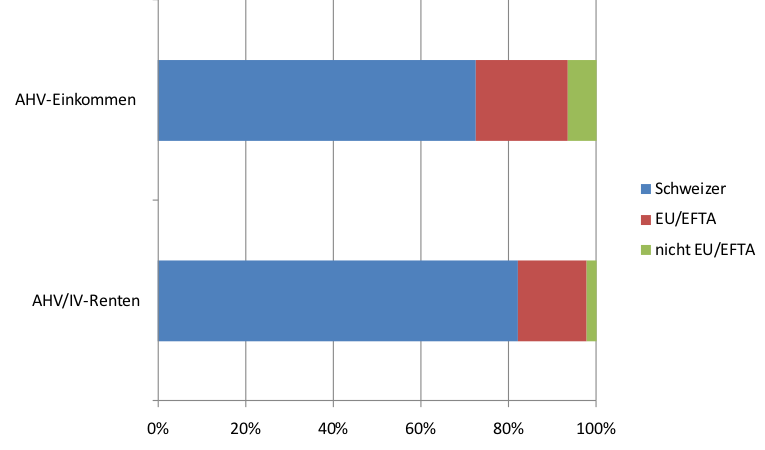
\includegraphics[width=0.7\textwidth]{images/AHV-Anteile.png}
	\end{center}
	\caption{Anteile der Einzahler/Bezüger nach Nationalität \cite[S. 72]{ADMIN:Bericht}}
	\label{fig:ahvanteil}
\end{figure}


